% !TeX root = bash.tex
\section{II. Back to Bash}
\begin{frame}
\frametitle{The CLI}

One of the ways we use Bash is by typing commands in the terminal, just like we just practiced. This 'text-in, text-out' way of talking to the computer is what we call the \textbf{CLI}, stands for \textbf{command line interface}, as opposed to a graphical user interface(GUI).

\begin{figure}[h]
    \centering
    \includegraphics[height=5cm]{cli}
\end{figure}
\end{frame}

\begin{frame}[fragile]
\frametitle{Body of a command}
\begin{lstlisting}[language=bash]
# Just an example
$ some_command some_file.txt -o 10 --long-option
\end{lstlisting}
\begin{tabular}{ll}
    \tt{some\_command}            & Command or Executable file \\
    \tt{some\_file.txt}    & Argument to \tt{some\_command} \\
    \tt{-o}              & short option(flag) starts with \tt{-} \\
    \tt{10}               & Argument to \tt{-o}\\
    \tt{--long-option}        & long option(flag) starts with \tt{--} \\
\end{tabular}

\begin{block}{}
    Bash commands follow the convention above, though the command and flag names differ. 
\end{block}
\end{frame}

\begin{frame}[fragile]
\frametitle{Example of a command}
\begin{lstlisting}[language=bash]
# list all files but trash recursively in reverse
$ ls -Rr --ignore=trash
\end{lstlisting}
\begin{tabular}{ll}
    \tt{ls}             & Executable in \tt{\$PATH} \\
    \tt{-Rr}            & Two short options: \tt{-R -r} \\
    \tt{--ignore=}      & Long option \\
    \tt{trash}          & Argument to \tt{--ignore}
\end{tabular}
\begin{block}{Notes}
    \begin{itemize}
        \item Not every program uses this \tt{--long-option} convention
        \item The equal sign after \tt{--ignore} is optional in this command
    \end{itemize}
\end{block}
\end{frame}

\begin{frame}[fragile]
\frametitle{I can't possibly remember all \tt{--this} and \tt{--that}!}
You don't need to! Try:

\begin{lstlisting}[language=bash]
$ man ls
$ ls --help
\end{lstlisting}
\vspace{0.5em}

Or search \url{https://man.archlinux.org/man/ls.1} and \url{https://man7.org/linux/man-pages/man1/ls.1.html}

Or chatxxT, Gexxxi, etc. 
\end{frame}

\begin{frame}[fragile]
\frametitle{Challenge}
\begin{itemize}
    \item Read the man page for \tt{head}
    \item Experiment with files in \tt{02-cli/}
    \item Find a command to generate the following:
\end{itemize}
\begin{lstlisting}[language=bash]
==> p0.txt <==
MANIFESTO OF THE COMMUNIST PARTY.

==> p1.txt <==
I. BOURGEOIS AND PROLETARIANS.
\end{lstlisting}
\pause
\begin{block}{Solution}
\begin{lstlisting}[language=bash]
$ head -n1 -v p0.txt p1.txt
\end{lstlisting}
\end{block}
\end{frame}

\begin{frame}[fragile]
\frametitle{Learning by doing}
Inside \tt{02-cli/}, run:
\begin{lstlisting}[language=bash]
$ diff sway.1.conf sway.2.conf
\end{lstlisting}
Congratulations, you just learned how to use \tt{diff}!
\vspace{1em}

Now, what does this command do?
\begin{lstlisting}[language=bash]
$ comm -12 sway.1.conf sway.2.conf
\end{lstlisting}
\end{frame}

\begin{frame}
\frametitle{How Bash Executes a Command}
\begin{center}
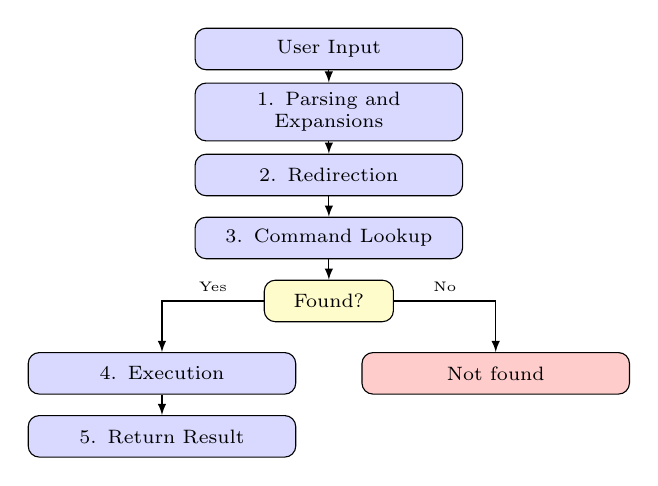
\begin{tikzpicture}[node distance=0.8cm, auto,
    block/.style={rectangle, draw, fill=blue!15, text width=9em, text centered, rounded corners, minimum height=1.5em, font=\scriptsize},
    decision/.style={rectangle, draw, fill=yellow!20, text width=4em, text centered, rounded corners, minimum height=1.5em, font=\scriptsize},
    line/.style={draw, -latex}]
    \node [block] (input) {User Input};
    \node [block, below of=input] (expand) {1. Parsing and Expansions};
    \node [block, below of=expand] (redir) { 2. Redirection};
    \node [block, below of=redir] (lookup) {3. Command Lookup};
    \node [decision, below of=lookup] (found) {Found?};
    \node [block, below left of=found, node distance=1.3cm, xshift=-1.2cm] (exec) {4. Execution};
    \node [block, below right of=found, node distance=1.3cm, xshift=1.2cm, fill=red!20] (error) {Not found};
    \node [block, below of=exec] (output) {5. Return Result};
    
    \path [line] (input) -- (expand);
    \path [line] (expand) -- (redir);
    \path [line] (redir) -- (lookup);
    \path [line] (lookup) -- (found);
    \path [line] (found) -| node [near start, above] {\tiny Yes} (exec);
    \path [line] (found) -| node [near start, above] {\tiny No} (error);
    \path [line] (exec) -- (output);
\end{tikzpicture}
\end{center}
\end{frame}

\begin{frame}
\frametitle{Wildcard}
\tt{*} is a character to match any number of (including zero) characters.

Bash will expand \tt{*} during Parsing and Expansions step.

\begin{block}{Note}
    Hidden paths will remain hidden unless you explicitly specify the dot:
    \tt{.*}
\end{block}

\begin{example}
    \begin{table}
        \centering
        \begin{tabular}{lcccc}
                       & \tt{a/}    & \tt{b/}    & \tt{a-copy.txt} & \tt{b.txt} \\ \hline
            \tt{*}     & \checkmark & \checkmark & \checkmark      & \checkmark \\
            \tt{a*}    & \checkmark &            & \checkmark      &            \\
            \tt{*.txt} &            &            & \checkmark      & \checkmark \\
        \end{tabular}
    \end{table}
\end{example}

\scriptsize{Technically it's called a glob pattern but who cares. Also there are other
weird symbols like \tt{?} or \tt{[]} but I swear \tt{*} is most of
us will ever use.}
\end{frame}

\begin{frame}
\frametitle{Shortcuts}

You could bind certain key presses to some useful commands.

Such as:
\begin{itemize}
    \item Use $\uparrow \downarrow$
    \item \tt{Ctrl-A}: move cursor to the beginning
    \item \tt{Ctrl-E}: move cursor to the end
    \item \tt{Ctrl-U}: delete everything to the left(or delete everything)
    \item \tt{Ctrl-K}: delete everything to the right
    \item \tt{Ctrl-C}: abort
    \item \tt{Ctrl-R}: incremental reverse search through command history
    \item \tt{Ctrl-L}: clear screen
\end{itemize}

\begin{block}{Note}{
   In bash, this is managed by \tt{bind}; and in zsh, this is managed by \tt{bindkey}. You could customize the binding.  
   \footnote{\tt{Ctrl-Q} and \tt{Ctrl-S} are binded with stream control. I recommend to turn it off.}    
    }
\end{block}
\end{frame}
